% vim: set tw=79

\documentclass[a4paper,10pt]{article}

\usepackage[utf8]{inputenc}
\usepackage{lipsum}
\usepackage{a4}
\usepackage[inline,nomargin]{fixme}
\usepackage{amsmath}
\usepackage{amssymb}
\usepackage{graphicx}
\usepackage{grffile}
\usepackage{url}
\usepackage{hyperref}
\usepackage{xcolor}
\usepackage{colortbl}
\usepackage{chngcntr}
\usepackage{caption}
\usepackage{subcaption}
\usepackage{amsmath}

% Python listing setup

\usepackage{color}
\usepackage[procnames]{listings}
\usepackage{textcomp}
\usepackage{setspace}
\usepackage{palatino}
\renewcommand{\lstlistlistingname}{Code Listings}
\renewcommand{\lstlistingname}{Code Listing}
\definecolor{gray}{gray}{0.5}
\definecolor{green}{rgb}{0,0.5,0}
\definecolor{lightgreen}{rgb}{0,0.7,0}
\definecolor{purple}{rgb}{0.5,0,0.5}
\definecolor{darkred}{rgb}{0.5,0,0}
\lstnewenvironment{python}[1][]{
\lstset{
language=python,
basicstyle=\ttfamily\small\setstretch{1},
stringstyle=\color{green},
showstringspaces=false,
alsoletter={1234567890},
otherkeywords={\ , \}, \{},
keywordstyle=\color{blue},
emph={access,and,as,break,class,continue,def,del,elif,else,%
except,exec,finally,for,from,global,if,import,in,is,%
lambda,not,or,pass,print,raise,return,try,while,assert},
emphstyle=\color{orange}\bfseries,
emph={[2]self},
emphstyle=[2]\color{gray},
emph={[4]ArithmeticError,AssertionError,AttributeError,BaseException,%
DeprecationWarning,EOFError,Ellipsis,EnvironmentError,Exception,%
False,FloatingPointError,FutureWarning,GeneratorExit,IOError,%
ImportError,ImportWarning,IndentationError,IndexError,KeyError,%
KeyboardInterrupt,LookupError,MemoryError,NameError,None,%
NotImplemented,NotImplementedError,OSError,OverflowError,%
PendingDeprecationWarning,ReferenceError,RuntimeError,RuntimeWarning,%
StandardError,StopIteration,SyntaxError,SyntaxWarning,SystemError,%
SystemExit,TabError,True,TypeError,UnboundLocalError,UnicodeDecodeError,%
UnicodeEncodeError,UnicodeError,UnicodeTranslateError,UnicodeWarning,%
UserWarning,ValueError,Warning,ZeroDivisionError,abs,all,any,apply,%
basestring,bool,buffer,callable,chr,classmethod,cmp,coerce,compile,%
complex,copyright,credits,delattr,dict,dir,divmod,enumerate,eval,%
execfile,exit,file,filter,float,frozenset,getattr,globals,hasattr,%
hash,help,hex,id,input,int,intern,isinstance,issubclass,iter,len,%
license,list,locals,long,map,max,min,object,oct,open,ord,pow,property,%
quit,range,raw_input,reduce,reload,repr,reversed,round,set,setattr,%
slice,sorted,staticmethod,str,sum,super,tuple,type,unichr,unicode,%
vars,xrange,zip},
emphstyle=[4]\color{purple}\bfseries,
upquote=true,
morecomment=[s][\color{lightgreen}]{"""}{"""},
commentstyle=\color{red}\slshape,
literate={>>>}{\textbf{\textcolor{darkred}{>{>}>}}}3%
         {...}{{\textcolor{gray}{...}}}3,
procnamekeys={def,class},
procnamestyle=\color{blue}\textbf,
framexleftmargin=1mm, framextopmargin=1mm, frame=shadowbox,
rulesepcolor=\color{blue},#1
}}{}



%\counterwithin{figure}{subsection}
%\counterwithin{table}{subsection}

%\setlength{\parindent}{0.0in}
%\setlength{\parskip}{0.1in}

\newcommand{\varopt}[1]{\textsc{#1}}
\newcommand{\numbots}{4}
\newcommand{\foodmass}{0.05}
\newcommand{\lightintensity}{0.01}

% Warning: these two are tightly coupled!
\newcommand{\tickinterval}{100 ms}
\newcommand{\tickspersecond}{10}



\title{
    IT - 3708 Sub-Symbolic AI Methods \\
    Homework Exercise 4\\
    ~\\
    \emph{Investigating Swarm Behaviour in Webots}
}
\author{
    Edvard K. Karlsen \\
    \texttt{edvardkk@stud.ntnu.no}
    \and
    Magne Vikjord \\
    \texttt{magnevan@stud.ntnu.no}
    \and
    Jonas Asmundsen \\
    \texttt{jonasbal@stud.ntnu.no}
}
\date {}


\begin{document}

\maketitle

\section{Introduction}
For the final project in IT 3708, we have designed and implemented a robot
controller based on Rodney Brooks' \emph{subsumption
architecture}~\cite{brooks1986}.  We have tested the
\emph{e-pucks}~\cite{bonani2009} in a collaborative box-pushing task simulated
in the Webots development environment.  

The intended box pushing behavior draws inspiration from the swarm behaviour
observed in ants during food retrieval.  The idea is to create a decentralized
system invoking group behavior through simple mechanisms which if successful,
leads to an emergent self-organized behaviour.

The rest of this report is structured as follows. In Section~\ref{sec:a1} we
give a brief overview of our system (Deliverable A1).  Further, in
Section~\ref{sec:a2} we describe our control system, and discuss its observed
behavior (Deliverable A2). Then, in Section~\ref{sec:b1} we discuss possible
improvements to the system (Deliverable B1). Finally, in Section~\ref{sec:b2}
we present out implementation of the improvements, and discuss how they
improved the e-puck's performance in the simulation (Deliverable B2).

\begin{figure}[!h]
  \centering
  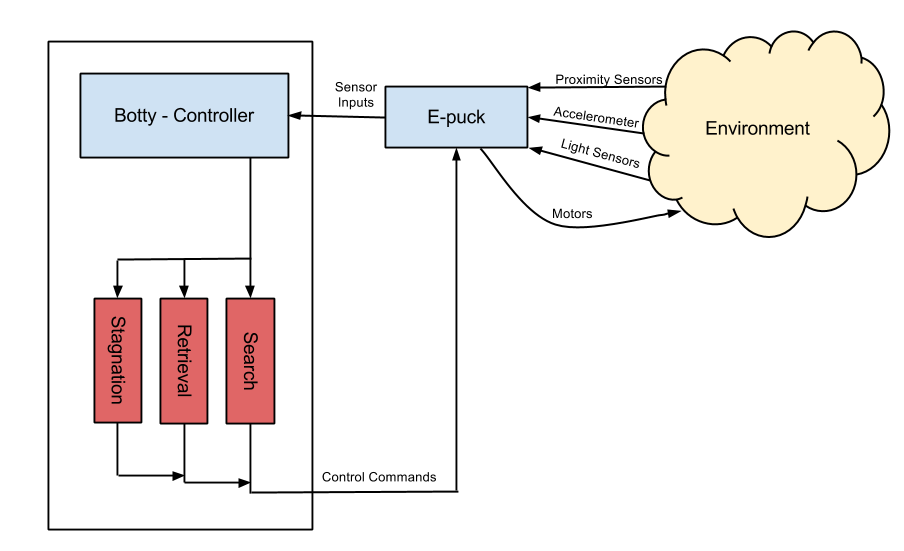
\includegraphics[width=0.99\textwidth]{%
    models/SubSym Proj 4 architecture.png}
    \caption{Overview of the e-puck control system}
  \label{fig:architecture}
\end{figure}

\section{System overview}
\label{sec:a1}

Figure~\ref{fig:architecture} illustrates the main components of our system.
In the figure, `environment' can be interpreted as the Webots simulation
world.

\subsection{Changes to the simulation world}
We tried to emulate our world to behave as closely to the live demonstration
we were given of the e-pucks swarm. With this aim in mind, we made the
following changes to the simulation world:

\begin{itemize}
    \item Removed all loose solids from the world except for one, which will
    become our food.
    \item Added physics to the food, and set the mass to \foodmass.
    We found this to be a good number for our basic tests as it
    requires two or more bots to be cooperating to push the box.
    \item Added a point light to the food with intensity \lightintensity.
    \item Removed all ambient lighting, and all other point lights. (Thus, the
    only remaining light source is the food.)
    \item Increased the number of e-pucks to \numbots.
    \item Reduced the tick interval to \tickinterval.
\end{itemize}


\subsection{E-puck control system}
\label{sec:a2}

We based our controller on the subsumption architecture that was used for
CRABS~\cite{berg2011}. The most primitive layer deals with \emph{searching}
the environment. The second layer is concerned with \emph{retrieval}. The most
sophisticated layer deals with \emph{stagnation} during the retrieval task.

\subsubsection{Behavior selection}
The layer/behavior-selection component of a subsumption-based system can be
implemented in many ways -- from ad-hoc solutions with explicit, highly
coupled, communication between layers, to general network graphs with
arbitrary suppression edges. We chose a compromise between simplicity and
flexibility: we use a single list of control layers sorted by ascending
sophistication. Each time we choose an action, we iterate through the list of
layers, and choose the action proposed by the most sophisticated suppressing
layer (or the most primal action, if no higher layers opt to suppress). 

The following Python-style pseudo code shows the outline of the
bot's control system (see \texttt{botty.py}).

\begin{python}
def run_botty(self):
    self.layers = [
        SearchLayer(),
        RetrievalLayer(),
        StagnationLayer()
    ]

    while True:
        self.tick()

def tick(self):
    proximities = self.get_proximities()
    lights      = self.get_lights()
    speed       = self.get_speed()

    output = None
    for each layer in self.layers:
        proposed_output, should_supress = layer.act(proximities, 
                                                    lights, speed)

        if output is None or should_supress:
            output = proposed_output

    self.move_wheels(output)
\end{python}

As is seen, each layer implements a general interface: 
\begin{python}
def act(self, proximities, lights, speed):
    # return two-tuple 
    # (output power), should_supress
\end{python}

\subsubsection{Search}
The search layer is built as a simple state-based random explorer, which also
tries to avoid crashing into walls.  This layer never suppresses (as it is the
most primitive). 

The exploration function is functionally similar to the following pseudo-code:

\begin{python}
def find_speed(proximities):
    prox_right, prox_left = proximities[:3], proximities[5:]

    # Check for obstacles
    if any(p > DIST_THRESH for p in prox_right+prox_left):
        tot         = sum(prox_right + prox_left)
        left_power  = sum(prox_left)  / tot
        right_power = sum(prox_right) / tot
        return left_power, right_power
    else:
        # No obstacles, continue in set random direction,
        # or, with random probability, choose a new direction
        if random() < PROB_CHANGE_DIR:
            self.rand_move_dir = (
                uniform(.5, 1.0), 
                uniform(.5, 1.0)
            )
        return self.rand_move_dir
\end{python}

The gist of the code is: If there are obstacles nearby, the bot should try
to avoid them. Otherwise, it will just continue in a set random motion, with
some chance of choosing a new direction (with our current parameter choice, a
direction change can be expected after 2-3 seconds). 

\subsubsection{Retrieval}
The retrieval layer mainly uses the light sensor to detect the presence of a
food source nearby, which when detected, it will home in on, and push.

The retrieval layer will begin suppressing as soon as it detects a light
signal over a certain threshold. When light is detected it will rotate clockwise until 
the light is the strongest right in front of the robot (presumably that's where 
the food is), and then move straight ahead to push it.

\subsubsection{Stagnation}
The stagnation layer is tasked with identifying stagnation, which is when a 
bot is trying to push a target, but for some reason fails to do so and does 
not move. The method for deducing whether or not this has occurred utilizes 
all sensory value input available.

The layer will collect all sensory input values from the last 
{\tickspersecond} iterations.  

For each sensor, its {\tickspersecond} values are analyzed. If the difference 
between the maximum value of the sequence and the minimum value of the 
sequence is above a certain threshold, stagnation is not considered to be in 
effect. Stagnation will only occur if no sensor reports any significant change 
in value within the {\tickspersecond} most recent iterations.

The following pseudo-code shows this:

\begin{python}
def _has_stagnated(self):
    if len(self._prev_observations) < 10:
        return False

    (proximity_observations,
     light_observations,
     acceleration_observations) = zip(*self._prev_observations)

    # See if proximity has changed in recent past
    if any(abs(max(i_sensor_obs) - min(i_sensor_obs)) > 150
           for i_sensor_obs in zip(*proximity_observations)):
        return False

    # See if light has changed in recent past
    if any(abs(max(i_sensor_obs) - min(i_sensor_obs)) > 150
           for i_sensor_obs in zip(*light_observations)):
        return False

    # See if acceleration has changed in recent past
    if any(abs(max(i_sensor_obs) - min(i_sensor_obs)) > 0.1
           for i_sensor_obs in zip(*acceleration_observations)):
        return False

    # Nothing has changed in recent future
    # This is indicative of a stagnation
    return True
\end{python}

\subsection{Resulting behavior}
\label{sec:part-a behavior}

Using this system, the robots will often manage to push the box into one of
the corners, as seen in the timings in the table below. However our bots did
display some strange behaviors we might want to correct.

First of, our bots would sometimes loose sight of the box it it was
pushing near the corners of the box, or close to another bot. The result would
be that the bot would sometimes spin almost $360^\circ$ around, instead of
just making the small correction necessary. Another problems was that the
bots would in addition to pushing the food, push each other quite aggressively,
which seems to have at least three detrimental effects.
\begin{enumerate}
\item They would push
each other off the box, which both slows down progress, and sometimes
leads to a change in direction of the box. Sometimes the box would almost
make it to an edge before the robots would make a turn and start pushing
it towards another far away edge.
\item Often we couldn't adequately detect stagnation, because even if
the box itself was not moving, the robots would be nudging each other
continuously, which to our stagnation algorithm is equivalent to genuine
movement of the box.
\item By pushing with an angle and not directly towards the target, some of 
    the force exhibited by the bot is wasted on moving along it. With each bot 
    exerting a reduced amount of force on the target, more bots are necessary 
    to make it move.
\end{enumerate}

\begin{table}
    \centering
    \begin{tabular}{c|c|c|c|c|c}
        \textbf{Run}    & \textbf{1} & \textbf{2} & \textbf{3} &
        \textbf{4}      & \textbf{5}     \\ \hline
        \textbf{Time}   & 00:44 & 00:22 & 00:38 &
        \textsc{stagnated} & 01:12 \\
    \end{tabular}
    \caption{Run-time tests on the bot defined in Part A}
\end{table}


\section{Possible improvements}
\label{sec:b1}

\subsection{Aimed retrieval}

The retrieval layer works by rotating until it has determined that it is 
facing the target box. Once it faces the target, it will commence moving 
farward as long as it determines it is still facing the box. The problem with 
this is that the bot will rarely push directly on the box, but with an angle.  
This is not beneficial for several reasons, as mentioned above.

We have solved this with a technique which controls the motors and the 
direction of the bot by utilizing the two most-front light sensors. This 
technique will make sure that the bot is facing the light source is a highest 
possible degree. The following pseudo-code shows this:

\begin{python}
right, left = float(proximities[0]), float(proximities[7])

if max((right, left)) > DIST_THRESH:
    total = right + left
    l_wheel_speed, r_wheel_speed = left / total, right / total
else:
    l_wheel_speed, r_wheel_speed = 1, 1
\end{python}

\subsection{Least effort rotation}

The search for a target ends when the bot senses a light above a threshold in 
any direction. The box will then proceed with rotating in order to face the 
target. The rotation direction was initially static, making the bot rotate 
sub-optimally.

We sought to improve this and the way we did this was simply to calculate 
which side of the robot that was exposed to more light, indicating where the 
target is and rotate in that direction. The following pseudo-code shows this:

\begin{python}
l_light_exposure = sum(lights[i] for i in xrange(4))
r_light_exposure = sum(lights[i] for i in xrange(4,8))

if l_light_exposure < r_light_exposure:
    l_wheel_speed, r_wheel_speed = .3, -.3
else:
    l_wheel_speed, r_wheel_speed = -.3, .3
\end{python}

\subsection{Derived speed to determine stagnation}

Our way of identifying stagnation was based upon non-changing sensor values.  
However, in a large, messy, stagnated situation, with many bots surrounding 
the target, there will always be some jostling between the bots. This makes 
sure that the sensor values does not stay constant and thus preventing us from 
correctly identifying stagnation.

Ideally, we would define stagnation as the act of trying to push a target, but 
not changing position, IE. not having a speed. It so happens that we know the 
acceleration of the bots and with the following formula we can derive the 
speed of the bot.

$$\int a \,\mathrm{d}t = v$$

By creating a thread and constantly summarizing the experienced acceleration, 
we can derive the speed of the bot and use it to determine whether the bot has 
stagnated or not. As even the pseudo-code is rather large, we will not present 
it here, but the actual code can be viewed in
\texttt{swarm-epuck/controllers/botty/botty.py} and 
\texttt{swarm-epuck/controllers/botty/stagnation.py}.

\section{Implementing and evaluating the improvements}

We tested our improvements over a number of runs, and not only did we eliminate
all the unwanted behaviors  mentioned in section \ref{sec:part-a behavior}, we also managed 
to get run-times to generally be below half a minutes (except in certain stress tests).

Due to the changes in the stagnation algorithm, we observed the bots were able 
to discover stagnation even in cases where there would be a lot of jostling
between the robots like we had expected. Our improvements to the retrieval
algorithms also seemed to have the desired effect, in that they both
converged upon the box faster, and seemed to be able to push the box
in a much more stable manner.

While testing, we found that in addition to the times displayed in table
\ref{improved bot tests}, our robots used approximately 40 seconds to
solve a test case we created where robots began in a stagnated state,
with a single robot on each side. And between one and two minutes, when
we made the box heavier and added four more robots to the swarm.

\begin{table}[h]
    \centering
    \begin{tabular}{c|c|c|c|c|c}
        \textbf{Run}    & \textbf{1} & \textbf{2} & \textbf{3} &
        \textbf{4}      & \textbf{5}     \\ \hline
        \textbf{Time}   & 00:12 & 00:22 & 00:20 & 00:12 & 00:26 \\
    \end{tabular}
    \caption{Run-time tests on average cases for the improved bot.}
    \label{improved bot tests}
\end{table}

\begin{figure}[!h]
    \centering

    \begin{subfigure}[!h]{0.45\textwidth}
        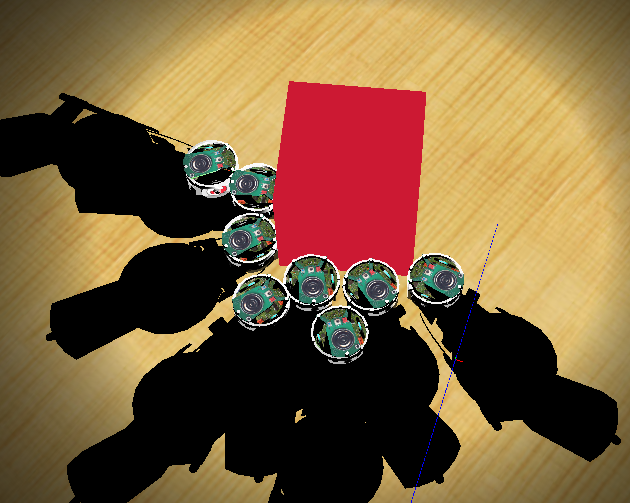
\includegraphics[width=\textwidth]{models/stresstest.PNG}
    \end{subfigure}
    \begin{subfigure}[!h]{0.45\textwidth}
        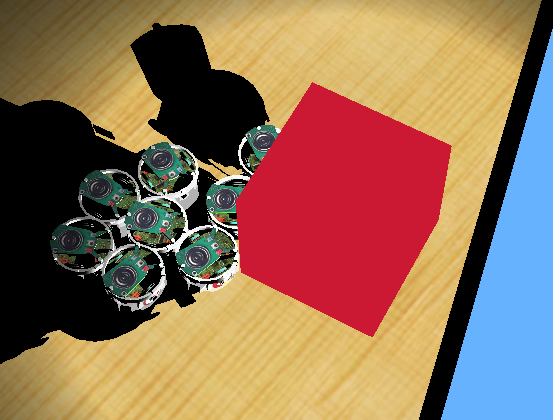
\includegraphics[width=\textwidth]{models/stresstest2.PNG}
    \end{subfigure}

    \caption{A group of eight e-pucks solving a $0.7$-mass box pushing task.
    To move a box with this mass, almost all the robots must take part in the
    pushing motion, and no robot can hinder it.}
\end{figure}


\label{sec:b2}


\bibliographystyle{plain}
\bibliography{refs} 

\end{document}
